\section{Datasets}\label{section:datasets}

All the datasets used in this study are publicly available. The selection process was aimed at finding a variety of different domains and complexity. Five datasets were selected, and each dataset is split into a training dataset and test dataset. If not defined in the dataset description, the split was done using $80:20$ proportions (\textit{training : test}). Besides the original split, each training dataset was additionally split into five training datasets. The second split creates the following structure for every dataset:

\begin{table}[ht]
\centering
\caption{Default dataset split structure}
\label{tab:dataset-split}
\begin{tabular}{|l|l|l|}
\hline
  & Training     & Test \\ \hline
A & 100\% * 80\% & 20\% \\ \hline
B & 80\% * 80\%  & 20\% \\ \hline
C & 60\% * 80\%  & 20\% \\ \hline
D & 40\% * 80\%  & 20\% \\ \hline
E & 20\% * 80\%  & 20\% \\ \hline
\end{tabular}
\end{table}

Table \ref{tab:dataset-split} can be read as \textit{"split B of the dataset X uses 80\% training dataset which consists of 80\% of the entire dataset, and full test dataset which consists of 20\% of the total dataset"}. If the class distribution is not constant, then splits of the train datasets are stratified. 

\begin{remark}\label{remark:performance-drop-while-train}
This split assumes that using a fraction of the training dataset for training will cause models to perform worse when tested on the same test dataset. It should simulate real-world issues with model accuracy and allow to experiment on none perfect models. The drop in the accuracy is not going to be linear because of the different complexities of each data domain.
\end{remark}

\subsection{Stanford Dogs}

The dataset created by Stanford University consists of dog pictures. It has 120 classes, and the train/test data split is defined by the authors. Class distribution is proportional between train and test splits. Dataset is slightly unbalanced, with the ratio between the least frequently occurring class and the most common class being $1.7$ (detailed class distribution available in appendix \ref{appendix:datasets:stanford-dogs}). The total number of images is 20580 (train: 16418, test: 4162). Examples from the datasets can be seen in Figure \ref{fig:stanford-dogs-example}.

\begin{figure}[ht]
    \centering
    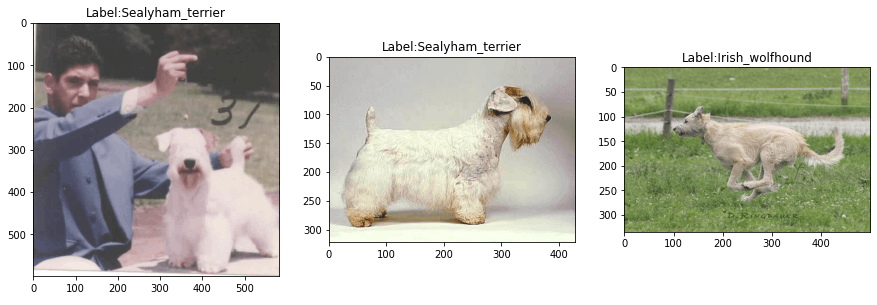
\includegraphics[width=0.65\textwidth]{experiments/datasets/dogs.png}
    \caption{Example images from in \textit{Stanford Dogs} \cite{stanford-dogs}}\label{fig:stanford-dogs-example}
\end{figure}

\subsection{Food 101}

The dataset consists of food pictures. It has 101 classes, and the train/test data split is defined by the authors. Classes are distributed proportionally, and each class has 750 examples in the train dataset and 250 examples in the test dataset, with the total number of images at 101000 (train: 75750, test: 25250). Examples from the datasets can be seen in Figure \ref{fig:food101-example}.

\begin{figure}[ht]
    \centering
    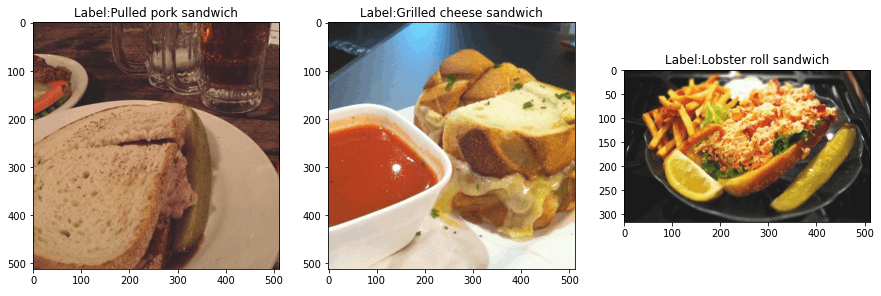
\includegraphics[width=0.65\textwidth]{experiments/datasets/food101.png}
    \caption{Example images from in \textit{Food 101} \cite{food101}}\label{fig:food101-example}
\end{figure}

\subsection{Edible wild plants}

The dataset consists of edible wild plants pictures. It has 62 classes, and the train/test data split is defined by the authors. Class distribution differs between train and test splits. Train dataset is highly unbalanced, with the ratio between the least frequently occurring class and the most common class being $21$ (detailed class distribution available in appendix \ref{appendix:datasets:edible-plants}). The unbalance is caused by 3 major classes. The rest of the dataset has the same ratio equal to $3$. The test dataset is balanced with $5$ examples for each class. The total number of images is 6868 (train: 6558, test: 310). Examples from the datasets can be seen in Figure \ref{fig:edible-plants-example}.

\begin{figure}[ht]
    \centering
    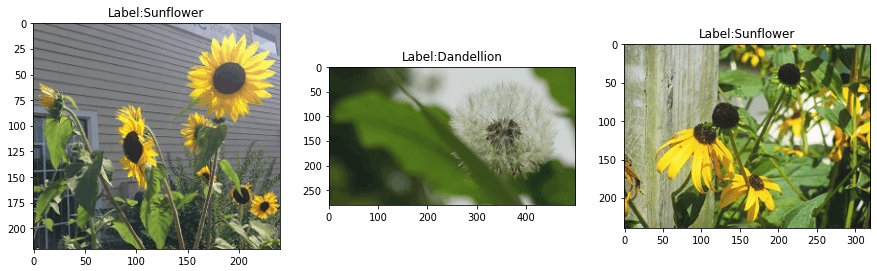
\includegraphics[width=0.65\textwidth]{experiments/datasets/wild-plants.png}
    \caption{Example images from in \textit{Edible wild plants} \cite{edible-wild-plants}}\label{fig:edible-plants-example}
\end{figure}

\subsection{Marvel Heroes}

The dataset consists of pictures from the Marvel Universe franchise. It has 8 classes, and the train/test data split is defined by the authors. Class distribution is proportional between train and test splits. Dataset is fairly balanced with ratio between the least frequently occurring class and the most common class being $1.12$ (detailed class distribution available in appendix \ref{appendix:datasets:marvel}). The total number of images is 3035 (train: 2584, test: 451). Examples from the datasets can be seen in Figure \ref{fig:marvel-example}.

\begin{figure}[ht]
    \centering
    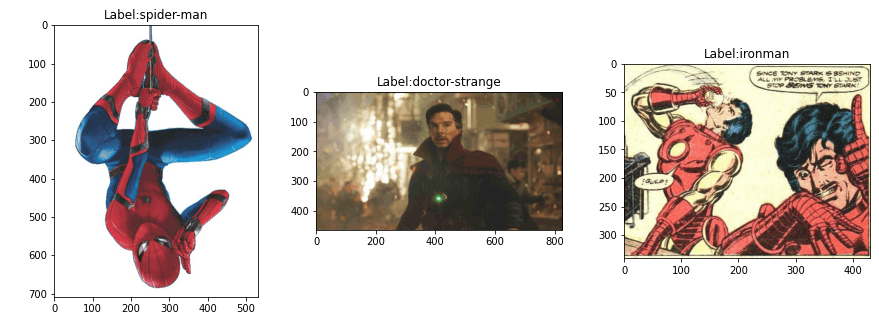
\includegraphics[width=0.65\textwidth]{experiments/datasets/marvel.png}
    \caption{Example images from in \textit{Marvel} \cite{marvel-heroes}}\label{fig:marvel-example}
\end{figure}

\subsection{Plants}

The dataset consists of plant pictures. It has 99 classes, and the train/test data split is defined by the authors. Class distribution is proportional between train and test splits (with the test dataset being slightly more balanced). Dataset is balanced with ratio between the least frequently occurring class and the most common class, being $7$ (detailed class distribution available in appendix \ref{appendix:datasets:plants}). The total number of images is 14670 (train: 13149, test: 1521). Examples from the datasets can be seen in Figure \ref{fig:plants-example}.

\begin{figure}[ht]
    \centering
    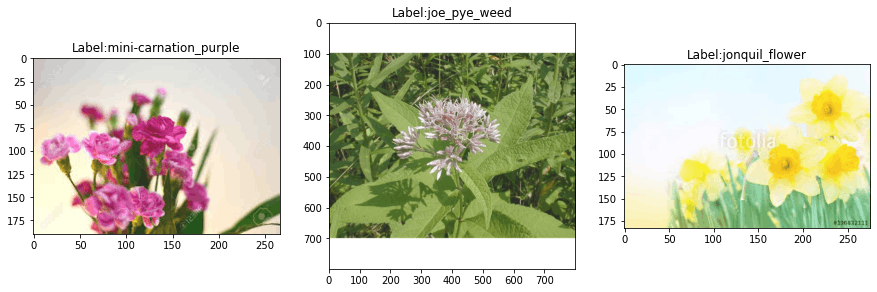
\includegraphics[width=0.65\textwidth]{experiments/datasets/plants.png}
    \caption{Example images from in \textit{Plants} \cite{plants-dataset}}\label{fig:plants-example}
\end{figure}